\documentclass[10pt]{article}
\usepackage[margin=2cm]{geometry}
\usepackage[T1]{fontenc}
\usepackage[utf8]{inputenc}
\usepackage{lmodern}
\usepackage{booktabs,longtable,graphicx,float,caption,array,xcolor}
\usepackage[hidelinks]{hyperref}
\captionsetup{font=small,labelfont=bf,skip=4pt}
\setlength{\parskip}{5pt}\setlength{\parindent}{0pt}
\setlength{\LTcapwidth}{\textwidth}
\title{Adjoint-DSMC Parameter Study\\[2pt]\large How seeds, particles, Fourier modes and the first step affect the drag optimiser}
\author{Hansel Carmona}
\date{1 October 2026}
\begin{document}
\maketitle

\section{Summary of results}
Within 10 Fourier modes the drag plateaus at about 69\% below the circle, but the gradient has not reached its noise floor and the shape is not converged in the number of Fourier modes.
Growing the number of random seeds during a run took the drag reduction from about 62\% to 69\%.
250k particles gave the same drag and search direction as 500k.
Running the optimiser's endgame mode with 1M particles from the best shape improved the drag by only about another 0.8\% and did not bring the gradient down to its noise floor.
The first-step size made negligible difference.
Adding more Fourier modes keeps lowering the drag, so with a fixed perimeter and a weak curvature penalty the ``optimal'' shape may depend on how many modes are allowed.

\begin{figure}[H]\centering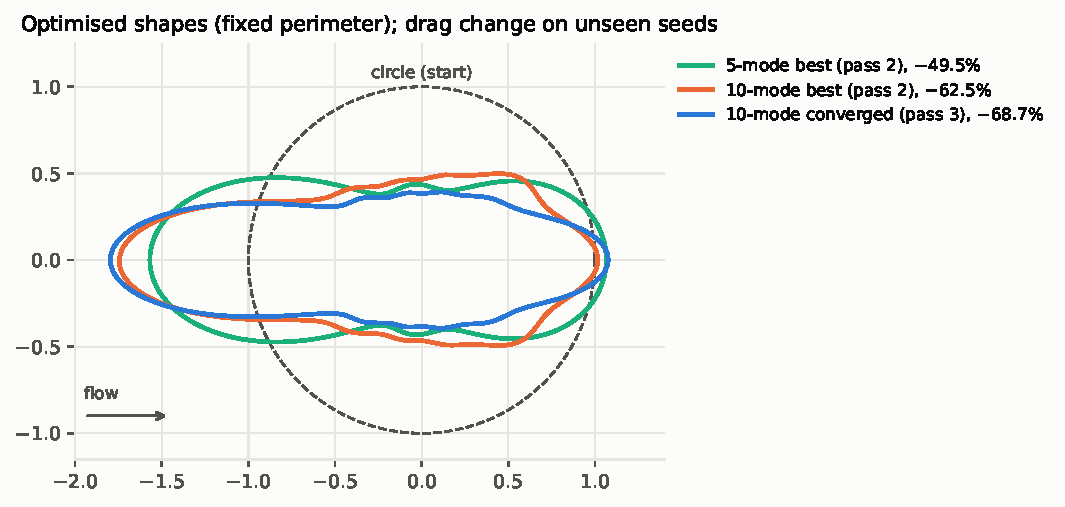
\includegraphics[width=0.92\textwidth,height=0.32\textheight,keepaspectratio]{summary/pass3_p3_shapes.pdf}\caption{\label{fig:shapes}This figure shows the best 5-mode and 10-mode shapes from pass 2 and the final 10-mode shape from pass 3, with their drag reductions on unseen seeds. All shapes have the same perimeter, and the gas flows from left to right.}\end{figure}

\section{Set-up}
Each iteration measures the drag and its gradient by averaging several independent random simulations (seeds), takes a step downhill, and checks that the drag really fell by more than the noise.
Table~\ref{tab:varied} lists the parameters that we varied, and every other setting was the same in every run.

\begin{table}[H]
\centering
\small
\caption{\label{tab:varied}The parameters that we varied. Every other setting was the same in every run.}
\begin{tabular}{l>{\raggedright\arraybackslash}p{6.6cm}>{\raggedright\arraybackslash}p{3.8cm}l}
\toprule
Parameter & What it controls & Values used & Baseline \\
\midrule
N\_AVG & The number of seeds averaged for each drag and gradient measurement. & 1, 2, 4, 8, 16 & 4 \\
N\_AVG\_MAX & The largest number of seeds a run may grow to. When it equals N\_AVG, the seed count is fixed. & = N\_AVG; 32 in passes 3 and 4 & = N\_AVG \\
N\_REF & The number of simulated particles in the channel. & 100k, 250k, 500k, 1M & 250k \\
N\_FOURIER & The number of Fourier modes that describe the shape. & 3, 5, 10, 20 & 10 \\
GRAD\_INIT\_FRAC & The size of the very first trial step, as a fraction of the size of the shape coefficients. & 0.01, 0.02, 0.05, 0.1, 0.2 & 0.05 \\
N\_ITER & The largest number of iterations a run may take. & 20, 50, 100; 30 in pass 4 & 20 \\
SEED0 & The first seed of a run. Replicates use separate seed sets. & 0, 100, 200, 300, 400 & 0 \\
ENDGAME & A final phase of gradient steps that do not have to prove an improvement. & off; 10 steps in pass 4 & off \\
Starting shape & The shape a run starts from. & circle; pass-3 shape in pass 4 & circle \\
\bottomrule
\end{tabular}
\end{table}


\subsection{The four passes}
\textbf{Pass 1.} The first pass used a baseline of N\_REF = 250k, N\_AVG = 4, N\_FOURIER = 10, GRAD\_INIT\_FRAC = 0.05 and N\_ITER = 20, and it varied one parameter at a time: N\_AVG over 1, 2, 8 and 16, N\_REF over 100k, 500k and 1M, N\_FOURIER over 3, 5 and 20, and GRAD\_INIT\_FRAC over 0.01, 0.02, 0.1 and 0.2.
It also measured the gradient at two fixed shapes with 16 seeds at each of the four particle counts.
It was meant to check how strongly each parameter affects the noise and the first stage of an optimisation.

\textbf{Pass 2.} The second pass lengthened the runs to 50 iterations and repeated six settings three times each with independent seed sets (SEED0 = 0, 100 and 200).
The six settings were the baseline, N\_REF = 500k, N\_AVG = 1, N\_AVG = 8, GRAD\_INIT\_FRAC = 0.1 and N\_FOURIER = 5.
It was meant to check whether the differences seen in pass 1 survive longer runs, and how repeatable each result is.

\textbf{Pass 3.} The third pass let the number of seeds grow during a run: each run started with N\_AVG = 4 and doubled its seeds, up to N\_AVG\_MAX = 32, whenever it could no longer confirm an improvement.
It ran four replicates (SEED0 = 0, 100, 200 and 300) for up to 100 iterations with 250k particles and 10 modes.
It also measured the drag and gradient at the best shapes on 32 unseen seeds, tested whether more Fourier modes would still lower the drag, and re-measured every final shape on 16 unseen seeds.
It was meant to check where a run ends when noise no longer stops it, how reproducible that end point is, and whether the result depends on the particle count or the number of modes.

\textbf{Pass 4.} The fourth pass continued from the pass-3 shape with N\_REF = 1M, 16 seeds growing to 32, 30 iterations and 10 endgame steps.
It was meant to check whether more particles and the endgame mode could push past the plateau and bring the gradient down to its noise floor.

\section{Results}
\subsection{Overall}
Table~\ref{tab:heldout} and Figure~\ref{fig:heldout} show how far each setting got on seeds that no run had used.
The pass-3 runs, which let the seed count grow, reached the lowest drag.
The ranking reflects how far each run got before noise stopped it, not over-fitting, because every shape performs the same on unseen seeds as on its own seeds within about one percentage point.

\begin{table}[H]
\centering
\small
\caption{\label{tab:heldout}How far each setting got. The values are drag reductions relative to the circle, re-measured on 16 seeds that no run used. Each run's standard error is 0.1 to 0.2 percentage points. The last column gives the largest difference between the own-seed and unseen-seed values of any run in the setting.}
\begin{tabular}{lrrrr}
\toprule
Setting & Runs & Mean \% & Range \% & Largest own$-$unseen gap \\
\midrule
Pass 4: 1M, endgame, from the pass-3 shape & 1 & 68.9 & -- & -- \\
Pass 3: 250k, seeds grow 4 to 32, up to 100 iterations & 4 & 68.6 & 68.1--69.0 & 0.34 \\
Pass 2: 250k, 8 seeds, 50 iterations & 3 & 62.2 & 61.4--62.9 & 0.44 \\
Pass 2: 500k, 4 seeds, 50 iterations & 3 & 62.6 & 62.3--62.7 & 0.55 \\
Pass 2: first step 0.1, 4 seeds, 50 iterations & 3 & 60.0 & 59.6--60.4 & 0.30 \\
Pass 2: baseline (250k, 4 seeds), 50 iterations & 3 & 58.6 & 55.4--62.0 & 0.38 \\
Pass 2: 1 seed, 50 iterations & 3 & 51.8 & 50.4--53.7 & 1.02 \\
Pass 2: 5 modes, 50 iterations & 3 & 49.5 & 49.4--49.6 & 0.74 \\
Pass 1: 10 modes, every setting, 20 iterations & 12 & 51.8 & 50.2--53.5 & 0.46 \\
Pass 1: 5 modes, 20 iterations & 1 & 49.0 & -- & 0.23 \\
Pass 1: 3 modes, 20 iterations & 1 & 32.6 & -- & 0.27 \\
\bottomrule
\end{tabular}
\end{table}

\begin{figure}[H]\centering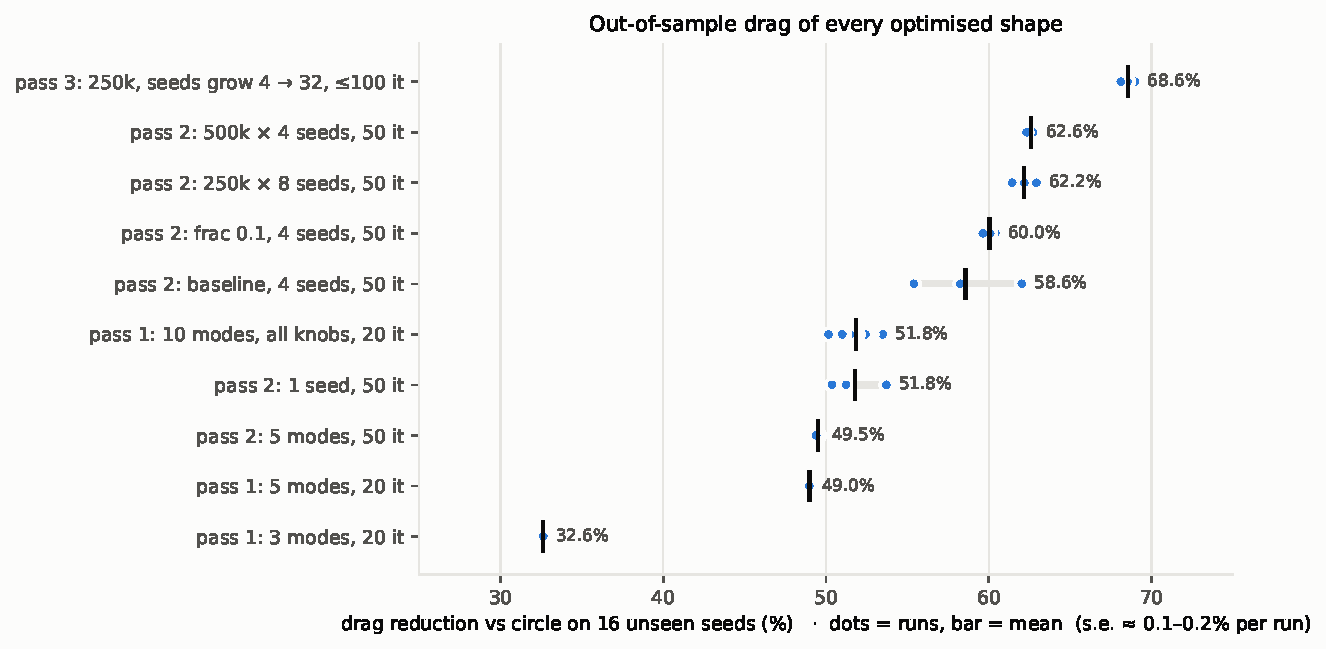
\includegraphics[width=0.92\textwidth,height=0.34\textheight,keepaspectratio]{summary/pass3_p3_heldout_by_setting.pdf}\caption{\label{fig:heldout}This figure shows the drag reduction of every optimised shape on 16 unseen seeds, grouped by setting. Each dot is one run, and the bar marks the mean.}\end{figure}

\subsection{Seeds}

Letting the seed count grow from 4 to 32 whenever the optimiser got stuck took the drag reduction from about 62\% to 69\% (Figure~\ref{fig:growth}).
A newly added seed must first settle at the current shape, because measured straight away it reads the drag 6.6\% too low.
Pass 3 therefore added seeds only through the line search, which lets new seeds settle first.

\begin{table}[H]
\centering
\small
\caption{\label{tab:seedsrun}Where runs with different seed settings stopped and how far they got. All of these runs used 10 modes and 250k particles, except for the row with 500k particles. The drag reductions were measured on unseen seeds.}
\begin{tabular}{llll}
\toprule
Seeds per gradient & Iterations reached & Why the runs stopped & Drag reduction \% \\
\midrule
1, fixed & 24--35 & noise limit & 50.4--53.7 \\
4, fixed & 27, 32, 50 & noise limit, iteration limit & 55.4, 58.3, 62.0 \\
8, fixed & 47--50 & iteration limit (one at the noise limit) & 61.4--62.9 \\
4, fixed, with 500k particles & 50 & iteration limit & 62.3--62.7 \\
4 $\to$ 32, growing & 81--100 & noise limit at 32 seeds, iteration limit & 68.1--69.0 \\
\bottomrule
\end{tabular}
\par\smallskip{\footnotesize\raggedright Four seeds with 500k particles average the same total number of simulated particles per measurement as eight seeds with 250k particles (2 million). The two settings therefore have about the same noise, and they reached the same place.\par}
\end{table}

\begin{table}[H]
\centering
\small
\caption{\label{tab:seedsneed}How many seeds are needed just to see the gradient. The second column is the scatter of one seed's gradient divided by the size of the mean gradient. The third column is the number of seeds that makes the gradient at least twice its standard error.}
\begin{tabular}{lrr}
\toprule
Shape & One-seed scatter / $\|g\|$ & Seeds needed \\
\midrule
Circle (start) & 0.18 & 1 \\
Best pass-2 shape & 0.97 & 4--5 \\
Final pass-3 shape, 250k & 1.14 & 6 \\
Final pass-3 shape, 1M & 0.54 & 2 \\
\bottomrule
\end{tabular}
\par\smallskip{\footnotesize\raggedright At the final shape, one of 32 seeds at 250k gave a gradient about 30 times the typical scatter, and it was left out of this table. Confirming that a small step lowered the drag needs many more seeds than seeing the gradient.\par}
\end{table}

\begin{figure}[H]\centering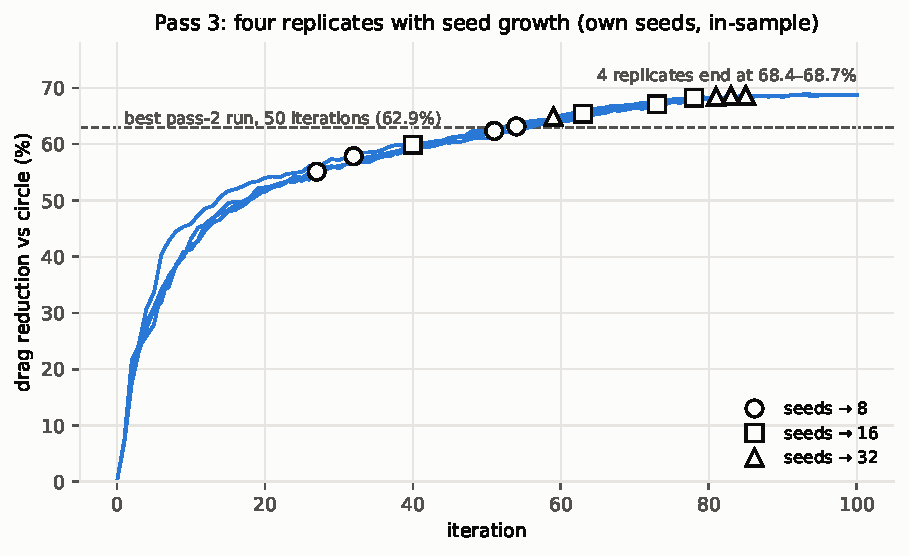
\includegraphics[width=0.92\textwidth,height=0.30\textheight,keepaspectratio]{summary/pass3_p3_growth_trajectories.pdf}\caption{\label{fig:growth}This figure shows the drag reduction against iteration for the four pass-3 replicates on their own seeds. The markers show where each run doubled its seeds instead of stopping.}\end{figure}

\subsection{Particles}
More particles reduce the noise at almost exactly the expected rate (Table~\ref{tab:noiseN}), so increasing particles or seeds yields the same result.
In pass 2, 500k particles with 4 seeds and 250k particles with 8 seeds reached nearly the same shape and drag (62.6\% and 62.2\%).
The particle count also has a floor for correctness (Table~\ref{tab:bias}).
At 100k the drag is right, but the search direction is slightly wrong, while at 250k and 500k both agree.
At the thin final shape, 1M particles sees about five times more pull on the finest mode than 250k does, so fine detail needs more particles.

\begin{table}[H]
\centering
\small
\caption{\label{tab:noiseN}How the gradient noise and the cost depend on the particle count. The noise is the scatter of one seed's gradient divided by the gradient's size, measured with 16 seeds in pass 1. At the circle it falls as $N^{-0.46}$, close to the ideal $N^{-1/2}$.}
\begin{tabular}{lrrrr}
\toprule
Particles & Noise, circle & Noise, stretched & s per seed-iteration & s per 100k particles \\
\midrule
100k & 25.1\% & 20.5\% & 41 & 41 \\
250k & 17.7\% & 17.0\% & 112 & 45 \\
500k & 11.4\% & 17.6\% & 163 & 33 \\
1M & 9.1\% & 7.6\% & 308 & 31 \\
\bottomrule
\end{tabular}
\end{table}

\begin{table}[H]
\centering
\small
\caption{\label{tab:bias}Whether the particle count biases the result. Each row measures the same fixed shape with two particle counts on the same unseen seeds. The drag is given per $10^5$ particles so that the counts can be compared. Two search directions count as the same when they differ by no more than their noise.}
\begin{tabular}{llrll}
\toprule
Comparison & Shape & Drag per $10^5$ particles & Same drag? & Same search direction? \\
\midrule
100k vs 500k & best pass-2 shape & 992 vs 993 & yes & no \\
100k vs 250k & best pass-2 shape & 992 vs 989 & yes & no \\
250k vs 500k & best pass-2 shape & 989 vs 993 & yes & yes \\
250k vs 1M & final pass-3 shape & 827 vs 826 & yes & yes, except the finest mode \\
\bottomrule
\end{tabular}
\par\smallskip{\footnotesize\raggedright At the final shape, 250k and 1M agree on the overall gradient, but in the finest mode $a_{10}$ 1M sees about five times more pull. The comparisons leave out a few seeds with extreme gradients, which would otherwise hide real differences.\par}
\end{table}


\subsection{Fourier modes}
More shape detail keeps lowering the drag (Table~\ref{tab:modes}).
At the optimised 10-mode shape, the gradient in modes 11--20 is seven to eight times the gradient in modes 1--10.
Stepping the shape into those modes lowered the drag on unseen seeds by up to 5.6\% (Table~\ref{tab:probes} and Figure~\ref{fig:probes}).
The same test on the 5-mode shape correctly predicted that 10 modes would do better.
The gain does not come from the body shrinking, because its height changed by only 0.6\%.
The result is therefore not converged in the number of modes.

\begin{table}[H]
\centering
\small
\caption{\label{tab:modes}The best drag reduction on unseen seeds for each number of Fourier modes.}
\begin{tabular}{ll>{\raggedright\arraybackslash}p{9.6cm}}
\toprule
Modes & Drag reduction \% & Notes \\
\midrule
3 & 32.6 & This was measured in pass 1, and the shape is too coarse. \\
5 & 49.5 & Three pass-2 replicates agree closely, and they stop after about 20 iterations. \\
10 & 62.5, then 68.7 & The first value is after 50 iterations, and the second is the pass-3 plateau. \\
20 & about 10 (own seeds) & Starting from the circle, the run stopped after 3 iterations, because the extra modes carry only noise there. \\
\bottomrule
\end{tabular}
\end{table}

\begin{table}[H]
\centering
\small
\caption{\label{tab:probes}What happens when an optimised shape is given extra modes. Each shape is stepped by $t$ into the modes it did not use, and its drag is re-measured on the same 16 unseen seeds. The change in the curvature penalty is shown in brackets.}
\begin{tabular}{lll}
\toprule
Step $t$ & 10-mode shape + modes 11--20, drag change \% & 5-mode shape + modes 6--10, drag change \% \\
\midrule
0.0025 & $-1.97 \pm 0.35$ (-4) & -- \\
0.005 & $-4.13 \pm 0.34$ (-5) & $-2.19 \pm 0.44$ (-5) \\
0.01 & $-5.57 \pm 0.29$ (+7) & $-5.21 \pm 0.40$ (-8) \\
0.02 & $-2.23 \pm 0.42$ (+78) & $-8.69 \pm 0.33$ (-7) \\
0.04 & -- & $-11.28 \pm 0.43$ (+18) \\
\bottomrule
\end{tabular}
\par\smallskip{\footnotesize\raggedright At the best pass-2 shape the gradient in modes 11--20 is about seven times the gradient in modes 1--10, and at the final pass-3 shape it is about eight times larger.\par}
\end{table}

\begin{figure}[H]\centering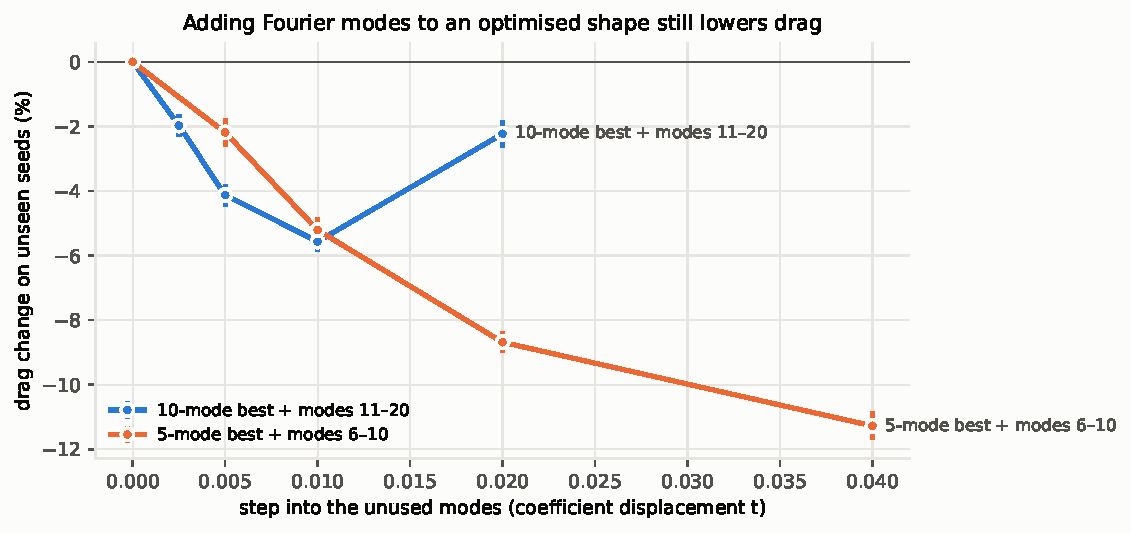
\includegraphics[width=0.92\textwidth,height=0.28\textheight,keepaspectratio]{summary/pass3_p3_mode_probes.pdf}\caption{\label{fig:probes}This figure shows how the drag changes when the optimised shapes are stepped into the modes they did not use. The drag was re-measured on unseen seeds, and the error bars are $\pm 1$ standard error.}\end{figure}

\subsection{First-step size}
The first-step size only changes the first three or four iterations (Table~\ref{tab:frac}).
Small values waste a few iterations growing the step, and large values overshoot once and back off.
After that all runs take steps of the same size, and the final results differ only by where individual runs stopped.

\begin{table}[H]
\centering
\small
\caption{\label{tab:frac}The effect of the first-step size in pass 1. The objective equals 1 at the circle, and the last column is the drag reduction on unseen seeds after 20 iterations.}
\begin{tabular}{rrrrr}
\toprule
GRAD\_INIT\_FRAC & Objective after 1 iteration & After 5 & After 20 & Drag reduction \% \\
\midrule
0.01 & 0.988 & 0.772 & 0.496 & 51.5 \\
0.02 & 0.968 & 0.682 & 0.480 & 52.4 \\
0.05 & 0.931 & 0.696 & 0.488 & 51.8 \\
0.1 & 0.862 & 0.666 & 0.481 & 52.6 \\
0.2 & 0.804 & 0.634 & 0.468 & 53.5 \\
\bottomrule
\end{tabular}
\par\smallskip{\footnotesize\raggedright In pass 2, a first step of 0.1 averaged 60.0\% after 50 iterations against 58.6\% for 0.05. That difference comes from where individual runs stopped, not from the step size.\par}
\end{table}


\subsection{The optimised shape}
The optimiser mainly flattens the body along the flow (Figure~\ref{fig:shapes}).
The final shape is 2.87 long and 0.79 tall, against $2.0 \times 2.0$ for the circle, with a long rounded front, a sharper tail and shallow ripples along the top and bottom.
The four pass-3 replicates agree on every coefficient to within a standard deviation of 0.009 (Table~\ref{tab:coeffs}).
The stretch coefficient $a_2$ sits exactly at the optimiser's stretch limit of $0.6\,c_0$.

\begin{table}[H]
\centering
\small
\caption{\label{tab:coeffs}The shape coefficients from each pass. Pass 1 is the baseline after 20 iterations, pass 2 is its best shape, pass 3 is the mean $\pm$ standard deviation over four replicates, and pass 4 is the final 1M shape.}
\begin{tabular}{lrrrr}
\toprule
Coefficient & Pass 1 & Pass 2 & Pass 3 (4 runs) & Pass 4 \\
\midrule
$c_0$ & +0.820 & +0.728 & $0.649 \pm 0.008$ & +0.632 \\
$a_{1}$ & -0.039 & -0.091 & $-0.120 \pm 0.006$ & -0.137 \\
$a_{2}$ & +0.244 & +0.348 & $0.389 \pm 0.005$ & +0.379 \\
$a_{3}$ & -0.138 & -0.134 & $-0.111 \pm 0.002$ & -0.114 \\
$a_{4}$ & +0.065 & +0.141 & $0.201 \pm 0.006$ & +0.210 \\
$a_{5}$ & -0.084 & -0.088 & $-0.074 \pm 0.004$ & -0.072 \\
$a_{6}$ & +0.052 & +0.084 & $0.114 \pm 0.006$ & +0.124 \\
$a_{7}$ & -0.024 & -0.040 & $-0.041 \pm 0.002$ & -0.037 \\
$a_{8}$ & +0.047 & +0.054 & $0.060 \pm 0.003$ & +0.068 \\
$a_{9}$ & +0.001 & -0.011 & $-0.015 \pm 0.001$ & -0.013 \\
$a_{10}$ & +0.026 & +0.025 & $0.024 \pm 0.001$ & +0.028 \\
$b_1\ldots b_{10}$ & $\le 0.003$ & $\le 0.003$ & $|\mathrm{mean}| \le 0.001$ & $\le 0.001$ \\
\bottomrule
\end{tabular}
\par\smallskip{\footnotesize\raggedright Every mode is capped at $0.6\,c_0$ by the optimiser's stretch limit (A\_MAX\_FRAC). In passes 3 and 4, $a_2/c_0 = 0.600$, which is exactly at the cap. The sine coefficients $b_k$ stay near zero, so the shape stays symmetric about the flow axis.\par}
\end{table}


\subsection{Pushing further with 1M particles and the endgame}
To test whether more precision could break the plateau, pass 4 continued from the pass-3 shape with 1M particles and the endgame mode (Table~\ref{tab:pass4}).
The drag fell by only $0.84 \pm 0.27$\% more on unseen seeds, and the gradient did not shrink.
With the body pressed against the stretch limit, more particles, more seeds and the endgame cannot move it much further.

\begin{table}[H]
\centering
\small
\caption{\label{tab:pass4}What happened in pass 4, which continued from the pass-3 shape with 1M particles and the endgame mode.}
\begin{tabular}{l>{\raggedright\arraybackslash}p{12.2cm}}
\toprule
Aspect & Result \\
\midrule
Normal phase & The run took 10 iterations and then reached the noise limit, even with 32 seeds. \\
Endgame (10 steps) & The objective stayed between 0.996 and 1.000 of its start, and the gradient stayed between 0.9 and 1.4 times its starting size. \\
Shape change & The shape moved by 0.031, which is about the spread between the pass-3 replicates, and $a_2$ stayed on the stretch limit. \\
Unseen seeds at 250k & The drag changed by $-0.69 \pm 0.49$\% against the pass-3 shape, which is not significant. \\
Unseen seeds at 1M & The drag changed by $-0.84 \pm 0.27$\% against the pass-3 shape, which is small but real. \\
Cost & The run took 6.3 hours on 16 cores. \\
\bottomrule
\end{tabular}
\end{table}


\end{document}
